\documentclass[11pt,a4paper]{article}
\usepackage[utf8]{inputenc}
\usepackage{amsmath, amssymb, amsthm}
\usepackage{geometry}
\usepackage{graphicx}
\usepackage{booktabs}
\usepackage{hyperref}
\usepackage{xcolor} % Required for defining custom colors
\usepackage{empheq} % Required for boxing numbered equations cleanly
\usepackage{algorithm}
\usepackage{algpseudocode}


\geometry{margin=1in}

\title{\textbf{Principal Component Analysis: Maximum Variance Formulation}}
\author{\textbf{Nishanka Das} \\ 
Department of Computer Science \\ 
Ramakrishna Mission Vivekananda Centenary College, Rahara
}

\date{\today}

% Define a command for the red box style
\newcommand{\redbox}[1]{\colorbox{red!10}{\setlength{\fboxrule}{1.2pt}\def\BorderColor{red}\fbox{#1}}}
% Alternative clean framework for empheq box
\newlength{\mytightbox}
\setlength{\mytightbox}{\fboxsep}

\begin{document}

\maketitle

\begin{center}
For any mistakes found please feel free to mail at: \\
\url{nishanka.das.rkmvcc@gmail.com}
\end{center}

\begin{abstract}
Principal Component Analysis (PCA) is an essential linear dimensionality reduction technique widely applied in data visualization, lossy compression, feature extraction, and noise reduction. This document presents a rigorous mathematical derivation of PCA following the Maximum Variance Formulation. Starting from first principles, we derive the optimal projection of high-dimensional continuous data onto a lower-dimensional subspace such that the sample variance of the projected points is maximized. Furthermore, we prove that the optimal projection directions correspond to the leading eigenvectors of the data covariance matrix and formulate the complete procedure via formal algorithmic pseudocode. The simulation of the algorithm is illustrated here;
\begin{figure}[ht]
    \centering
    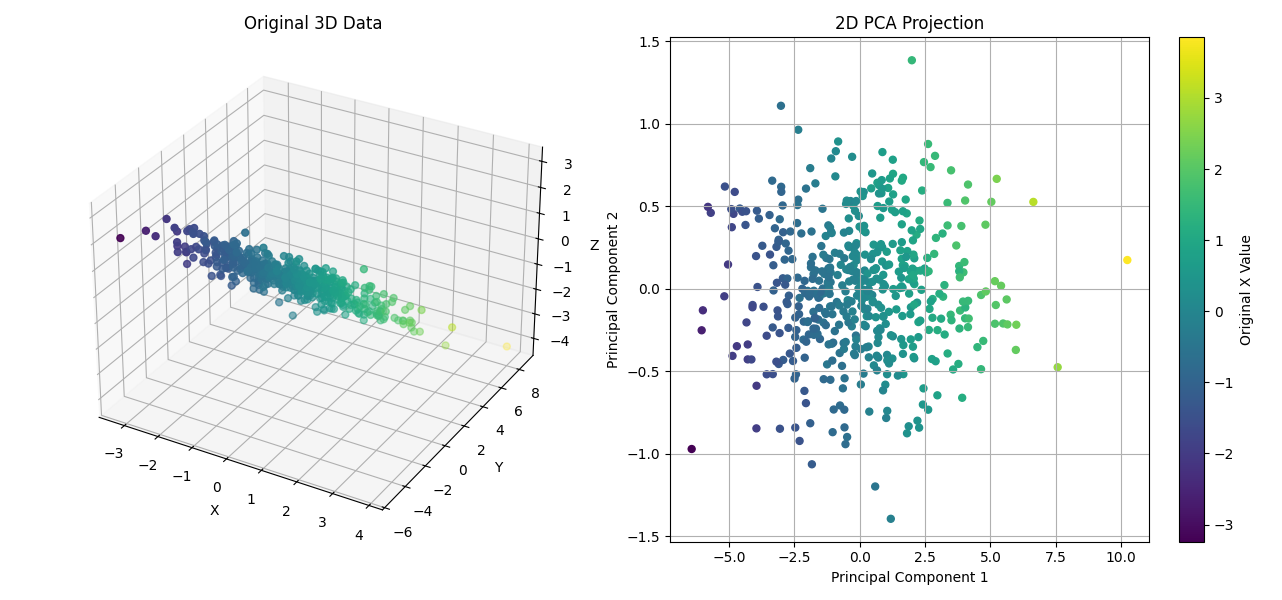
\includegraphics[width=0.75\textwidth]{Figure_2.png}
    \caption{PCA visualization}
    \label{fig:pca}
\end{figure}
\end{abstract}

\section{Formal Mathematical Formulation of PCA}
Consider an $N \times D$ data matrix $\mathbf{X}$ consisting of $N$ continuous real-valued observations $\{\mathbf{x}_1, \mathbf{x}_2, \dots, \mathbf{x}_N\}$, where each individual observation vector $\mathbf{x}_n \in \mathbb{R}^D$:
\begin{equation}
\mathbf{X} = 
\begin{pmatrix}
x_{11} & x_{12} & \cdots & x_{1D} \\
x_{21} & x_{22} & \cdots & x_{2D} \\
\vdots & \vdots & \ddots & \vdots \\
x_{N1} & x_{N2} & \cdots & x_{ND}
\end{pmatrix}
\end{equation}

The primary objective of Principal Component Analysis (PCA) is to find a linear transformation that projects the dataset onto a lower-dimensional linear subspace of dimension $M < D$ while maximizing the sample variance of the projected data.

\subsection{Defining the One-Dimensional Projection Direction}
To construct the foundation of PCA, we begin by projecting the data onto a one-dimensional space ($M = 1$). The direction of this 1D subspace is defined by a $D$-dimensional vector $\mathbf{u}_1 \in \mathbb{R}^D$. Because we are solely concerned with spatial direction rather than scale, we impose the strict unit-norm normalization condition:
\begin{equation}
\mathbf{u}_1^T \mathbf{u}_1 = 1
\end{equation}

Each high-dimensional data observation $\mathbf{x}_n$ is orthogonally projected onto $\mathbf{u}_1$, yielding a scalar coordinate value given by the inner product $\mathbf{u}_1^T \mathbf{x}_n$.

\subsection{Formulating the Projected Variance}
The sample mean vector $\mathbf{\bar{x}} \in \mathbb{R}^D$ of the original unprojected observations is defined as:
\begin{equation}
\mathbf{\bar{x}} = \frac{1}{N}\sum_{n=1}^{N} \mathbf{x}_n
\end{equation}

Consequently, by the linearity of expectation and inner products, the sample mean of the projected scalar data coordinates is $\mathbf{u}_1^T \mathbf{\bar{x}}$. The total sample variance $\sigma_{\text{proj}}^2$ of the projected observations is defined as:
\begin{equation}
\sigma_{\text{proj}}^2 = \frac{1}{N}\sum_{n=1}^{N} \left\{ \mathbf{u}_1^T \mathbf{x}_n - \mathbf{u}_1^T \mathbf{\bar{x}} \right\}^2
\end{equation}

By factoring out the projection vector $\mathbf{u}_1$ from the squared term:
\begin{equation}
\left( \mathbf{u}_1^T \mathbf{x}_n - \mathbf{u}_1^T \mathbf{\bar{x}} \right)^2 = \left( \mathbf{u}_1^T (\mathbf{x}_n - \mathbf{\bar{x}}) \right) \left( \mathbf{u}_1^T (\mathbf{x}_n - \mathbf{\bar{x}}) \right)^T = \mathbf{u}_1^T (\mathbf{x}_n - \mathbf{\bar{x}})(\mathbf{x}_n - \mathbf{\bar{x}})^T \mathbf{u}_1
\end{equation}

Substituting this back into the variance expression yields:
\begin{equation}
\sigma_{\text{proj}}^2 = \mathbf{u}_1^T \left[ \frac{1}{N}\sum_{n=1}^{N} (\mathbf{x}_n - \mathbf{\bar{x}})(\mathbf{x}_n - \mathbf{\bar{x}})^T \right] \mathbf{u}_1 = \mathbf{u}_1^T \mathbf{S} \mathbf{u}_1
\end{equation}
where $\mathbf{S}$ represents the symmetric $D \times D$ sample covariance matrix:
\begin{equation}
\mathbf{S} = \frac{1}{N}\sum_{n=1}^{N} (\mathbf{x}_n - \mathbf{\bar{x}})(\mathbf{x}_n - \mathbf{\bar{x}})^T
\end{equation}

\subsection{Constrained Optimization via Lagrange Multipliers}
Our objective is to maximize the projected variance function $\mathbf{u}_1^T \mathbf{S} \mathbf{u}_1$ with respect to $\mathbf{u}_1$. To prevent the magnitude $\|\mathbf{u}_1\|$ from approaching infinity, we apply the normalization constraint $\mathbf{u}_1^T \mathbf{u}_1 = 1$ using a Lagrange multiplier denoted by $\lambda_1$:
\begin{equation}
\mathcal{L}(\mathbf{u}_1, \lambda_1) = \mathbf{u}_1^T \mathbf{S} \mathbf{u}_1 + \lambda_1 \left(1 - \mathbf{u}_1^T \mathbf{u}_1\right)
\end{equation}

To locate the critical stationary points, we differentiate $\mathcal{L}$ with respect to $\mathbf{u}_1$. Recalling matrix calculus identity $\frac{\partial}{\partial \mathbf{x}}(\mathbf{x}^T \mathbf{A} \mathbf{x}) = 2\mathbf{A}\mathbf{x}$ for symmetric matrix $\mathbf{A}$:
\begin{equation}
\frac{\partial \mathcal{L}}{\partial \mathbf{u}_1} = 2\mathbf{S}\mathbf{u}_1 - 2\lambda_1 \mathbf{u}_1 = 0
\end{equation}

Dividing by $2$ yields the fundamental matrix eigenvalue equation:
\begin{equation}
\mathbf{S}\mathbf{u}_1 = \lambda_1 \mathbf{u}_1
\end{equation}

This proves that $\mathbf{u}_1$ must be an **eigenvector** of the data covariance matrix $\mathbf{S}$. Left-multiplying both sides by $\mathbf{u}_1^T$ and applying the unit-norm constraint $\mathbf{u}_1^T \mathbf{u}_1 = 1$:
\begin{equation}
\mathbf{u}_1^T \mathbf{S} \mathbf{u}_1 = \lambda_1 \mathbf{u}_1^T \mathbf{u}_1 = \lambda_1
\end{equation}

Thus, the projected sample variance is precisely equal to the eigenvalue $\lambda_1$. To maximize this variance, $\mathbf{u}_1$ must be selected as the eigenvector corresponding to the **largest eigenvalue** $\lambda_1$. This directional vector $\mathbf{u}_1$ is defined as the **First Principal Component**.

\section{Generalization to $M$-Dimensional Subspaces}
To extend this formulation to a general $M$-dimensional linear projection space ($M < D$), additional principal component directions ($\mathbf{u}_2, \dots, \mathbf{u}_M$) are chosen incrementally. Each successive direction $\mathbf{u}_m$ is selected to maximize the projected variance subject to being mutually orthogonal to all previously established directions:
\begin{equation}
\mathbf{u}_i^T \mathbf{u}_j = 0 \quad \forall i \neq j \quad \text{and} \quad \mathbf{u}_m^T \mathbf{u}_m = 1
\end{equation}

Using Lagrange multipliers for multiple orthogonality constraints, it can be proven by induction that the optimal linear $M$-dimensional subspace preserving maximum variance is defined by the matrix of $M$ eigenvectors corresponding to the $M$ largest eigenvalues $(\lambda_1 \ge \lambda_2 \ge \dots \ge \lambda_M)$ of the covariance matrix $\mathbf{S}$.

The total variance retained by the $M$-dimensional subspace relative to the total variance in the original data is quantified by the proportion of variance explained:
\begin{equation}
\text{Explained Variance Ratio} = \frac{\sum_{i=1}^{M} \lambda_i}{\sum_{j=1}^{D} \lambda_j}
\end{equation}

The simulation of PCA is attached here with components of 128,64,32 and 16. 

\begin{figure}[ht]
    \centering
    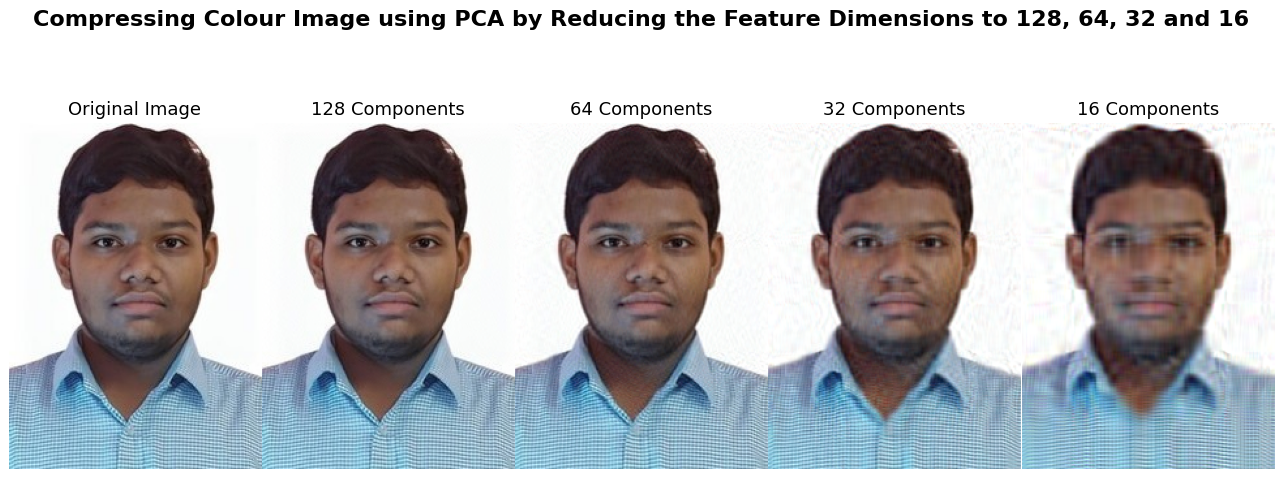
\includegraphics[width=0.75\textwidth]{Figure_1.png}
    \caption{PCA visualization for RGB image. To see the code and generate for your image \href{https://github.com/NishankaDas/ML-DL/blob/main/ML-DL/pca.py}{\textcolor{red}{Click Here} }}
    \label{fig:pca1}
\end{figure}
\section{Algorithmic Formalization}
The procedural execution of Principal Component Analysis is formally structured in Algorithm \ref{alg:pca}.

\begin{algorithm}[H]
\caption{Principal Component Analysis (Maximum Variance Formulation)}
\label{alg:pca}
\begin{algorithmic}[1]
\Require Data matrix $\mathbf{X} \in \mathbb{R}^{N \times D}$, Target dimensionality $M < D$
\Ensure Transformation matrix $\mathbf{U}_M \in \mathbb{R}^{D \times M}$, Dimensionality-reduced coordinates $\mathbf{Z} \in \mathbb{R}^{N \times M}$
\Procedure{PCA}{$\mathbf{X}, M$}
    \State $\mathbf{\bar{x}} \gets \frac{1}{N}\sum_{n=1}^{N} \mathbf{x}_n$ \Comment{Compute $D$-dimensional sample mean vector}
    \State $\mathbf{S} \gets \frac{1}{N}\sum_{n=1}^{N} (\mathbf{x}_n - \mathbf{\bar{x}})(\mathbf{x}_n - \mathbf{\bar{x}})^T$ \Comment{Construct $D \times D$ sample covariance matrix}
    \State $\{\lambda_i, \mathbf{u}_i\}_{i=1}^D \gets \text{EigenDecomposition}(\mathbf{S})$ \Comment{Solve $\mathbf{S}\mathbf{u}_i = \lambda_i \mathbf{u}_i$}
    \State Sort $\{\lambda_i, \mathbf{u}_i\}$ in descending order such that $\lambda_1 \ge \lambda_2 \ge \dots \ge \lambda_D$
    \State $\mathbf{U}_M \gets [\mathbf{u}_1, \mathbf{u}_2, \dots, \mathbf{u}_M]$ \Comment{Select top $M$ eigenvectors as matrix columns}
    \For{$n = 1$ to $N$}
        \State $\mathbf{z}_n \gets \mathbf{U}_M^T (\mathbf{x}_n - \mathbf{\bar{x}})$ \Comment{Project mean-centered point into $M$-dimensional space}
    \EndFor
    \State \Return $\mathbf{U}_M, \mathbf{Z}$
\EndProcedure
\end{algorithmic}
\end{algorithm}

\end{document}